\documentclass[a4paper]{article}
%\usepackage{fourier-otf}
\usepackage[utf8]{inputenc}
\usepackage{graphicx}
\usepackage{amsmath}
\usepackage{amsfonts}
\usepackage{float}
\usepackage{biblatex}
\addbibresource{bibliography.bib}
\usepackage{listings}
%\usepackage[square,sort,comma,numbers]{natbib}
\newtheorem{theorem}{Theorem}[section]
\usepackage{color}
\usepackage{makeidx}
\usepackage{titlepic}
\definecolor{mygreen}{rgb}{0,0.6,0}
\definecolor{mygray}{rgb}{0.5,0.5,0.5}
\definecolor{mymauve}{rgb}{0.58,0,0.82}
\lstset{ %
	backgroundcolor=\color{white},   % choose the background color
	basicstyle=\footnotesize,        % size of fonts used for the code
	breaklines=true,                 % automatic line breaking only at whitespace
	captionpos=b,                    % sets the caption-position to bottom
	commentstyle=\color{mygreen},    % comment style
	escapeinside={\%*}{*)},          % if you want to add LaTeX within your code
	keywordstyle=\color{blue},       % keyword style
	stringstyle=\color{mymauve},     % string literal style
}
\usepackage{hyperref}
\hypersetup{
  colorlinks   = true,    % Colours links instead of ugly boxes
  urlcolor     = black,    % Colour for external hyperlinks
  linkcolor    = black,    % Colour of internal links
  citecolor    = black      % Colour of citations
}
\title{Incontri tesi IIT}

\author{F.Bernardi - G.Fregiari - R.Sacco - G.Chiaravalli}







\begin{document}
		\maketitle
	\clearpage
	
	\clearpage
	
	\section{Incontro 1 (05/10/2021)}
	
	\subsection{Spiegazione dell'esperimento}
	
	L'esperimento di interbrain svolto sui topi si pone l'obiettivo di studiare l'attività cerebrale (attività del calcio intracellulare) in 3 tipi di cavie: \textbf{observer, neutral, altered}.\\
	Il topo observer è libero di muoversi in un'arena in cui, in due gabbie distinte, sono presenti anche i topi neutrale e alterato. Il topo è alterato se il suo \textit{affective state} è modificato in negativo (mancanza di acqua, topo stressed), o in positivo (dopo mancanza di acqua, acqua a volontà). \\
	 Gli obiettivi dell'esperimento possono essere molteplici: monitorare l'attività calcio nell'observer e vedere come cambia quando esso si trova in prossimità di neutrale e alterato, trovare pattern nell'accensione dei neuroni ecc... Si vuole inoltre studiare la \textit{sincronizzazione} neuronale: attività calcio simili tra due topi che interagiscono, ed eventuale imposizione del ritmo da parte di uno dei due (parte di interbrain, vedi articolo Kingsbury). \\
	L'esperimento consiste di 3 fasi:
	\begin{itemize}
		\item \textbf{homecage}: i topi sono in una gabbia, fermi, isolati dagli altri. Per 5 minuti si monitora l'attività calcio
		
		\item \textbf{habituation}: il topo observer è libero di girare per l'arena, ma senza poter iteragire con gli altri due. Si vuole vedere come è, in condizioni isolate, l'attività dell'observer e il suo movimento nell'arena, per 15 minuti
		
		\item \textbf{test}: il test vero e proprio con tutti e 3 i topi, per 15 minuti
		
	\end{itemize}
	
	
	\begin{figure}[H]
		\begin{center}
			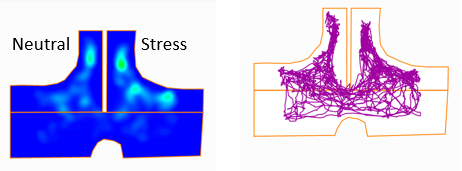
\includegraphics[scale=.80]{arena.png} 
		\end{center} 
		\caption{A sinistra l'arena con le due gabbie in corrispondenza dei nomi neutral e stressed. A destra il movimento effettuato dall'observer durante il test}
	\end{figure}

\newpage

\subsection{Inscopix e file excel}

Inscopix è l'azienda che produce i microscopi che inseriti nel topo, ne monitorano l'attività. Prima del test, viene iniettato nel topo un virus che reagisce con il calcio provocando fluorescenza. Tale fluorescenza viene misurata per ogni frame come $\frac{\Delta F}{F_b} = \frac{F(x,y,t)-F_b}{F_b}$, dove $F(x,y,t)$ è la fluorescenza misurata nel punto $(x,y)$ al tempo $t$, mentre $F_b$ è la fluorescenza baseline, scelta in genere come la media o la minima (vedi pag. 41 manuale). Dai video ottenuti lungo le 3 fasi dell'esperimento, attraverso diversi algoritmi di identififcazione, filtering ecc (vedi manuale), si producono diversi file excel, da analizzare su Matlab:
\begin{itemize}
	\item Un file per ognuno dei 3 topi con i tempi nella prima colonna e, nelle successive, ogni colonna per un neurone, che alla riga corrispondente a un tempo avrà il valore misurato  $\frac{\Delta F}{F_b}$. La prima riga dice se il neurone è preferibile da accettare o rifiutare a seguito del processing di inscopix
	
	\item  Due file tengono traccia della posizione dell'observer (uno durante l'habituation, uno durante il test), indicando le sue coordinate e la sua vicinanza o meno alle gabbie degli altri due topi con valori binari
	
	\item Un file contiene informazione sull'attività (sniffing) dell'observer in interazione con gli altri topi
	
\end{itemize}

\begin{figure}[H]
	\begin{center}
		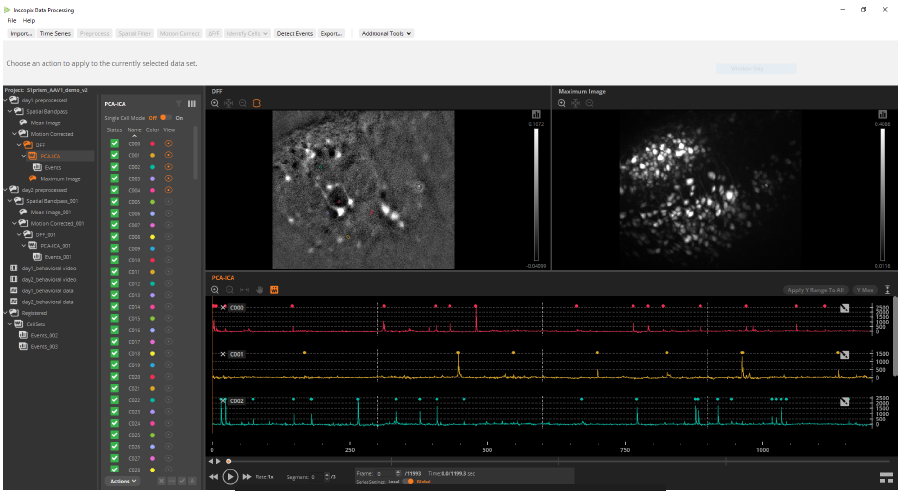
\includegraphics[scale=.60]{inscopix.png} 
	\end{center} 
	\caption{Esempio video processato da Inscopix}
\end{figure}

\newpage
\subsection{Discussione}

L'analisi del dataset può percorrere tantissime strade diverse. Si è per esempio discusso di:

\begin{itemize}
	\item Il metodo più adeguato per rappresentare l'attività del calcio estesa al singolo topo, anzichè a un singolo neurone. Una media semplice è sufficiente? Idea di considerare una media pesata per ogni neurone, dove i pesi vengono determinati in base a quanto il neurone è correlato all'interazione del topo con gli altri due (esempio, modello lineare generalizzato con attività dei neuroni come covariate, risposta come attività di sniffing verso un topo). così facendo si vede l'attività media del topo intesa come attività dei neuroni direttamente coinvolti nell' interazione (e magari sincronizzazione) \\
	(Non so se sta roba che ho scritto ha senso LOL)
	
	\item Riccardo suggerisce che, avendo l'attività calcio dell'observer,  possiamo pensarla come funzione che varia nello spazio, durante il test in cui l'observer si muove nell'arena. Così facendo possiamo per esempio plottarla nel dominio dato dall'arena stessa ed associare ad ogni punto dell'arena una concentrazione calcio, per poi vedere cosa succede nelle aree vicine ai topi neutrale e stressato
	
	\item In parallelo all'analisi dei dati, si può lavorare alla \textbf{modellistica del calcio}. Problema: tali modelli studiano i meccanismi intracellulari di bilancio del calcio, ma il microscopio non ha una risoluzione così elevata da fornire validazioni sperimentali. Greta C. suggerisce di pensare a ordini di grandezza più elevati, per esempio alla diffusione del calcio tra i neuroni della rete osservata. \\
	Non discusso ma lo dico ora: Fabrizio si chiede se è possibile comunque pensare  a un modello a "scatola chiusa", in cui ciò che succede all'interno del neurone lo si cerca di implementare da ciò che si è fatto in letteratura, ma in cui si personalizza al caso nostro focalizzandosi su ciò che il modello "scatola chiusa" prende dall'esterno per caratterizzare ogni singola simulazione dell'onda calcio (TBC).
\end{itemize}

Per quanto riguarda l'analisi dei dati, i primi passi saranno:

\begin{itemize}
	\item funzioni Matlab che scompongono il segnale nelle 3 fasi dell'esperimento dai file excel originali
	
	\item \textbf{ normalizzazione del segnale}, per esempio \textit{normalization z-score} $z = \frac{x - \mu}{\sigma}$ o \textit{min-max normalization} $x' = \frac{x - min(x)}{max(x) - min(x)}$
	
	\item \textbf{Statistica descrittiva} sul campione di dati: giù di medie, variabilità, boxplot e istogrammi
	
	\item \textbf{identificazione dei picchi} : quando possiamo considerare un neurone attivo? Una soluzione può essere considerare tutto ciò sopra a un certo valore come attività e tutto ciò sotto no, utilizzando come treshold, ad esempio, $ y = \mu + \sigma $, media del segnale + deviazione standard (tutto ciò che è sopra tale retta può andare a costituire un 1 in un vettore di 0/1 che ci dice per ogni neurone se esso è attivo)
	
	\item \textbf{Correlazioni tra neuroni}: c'è qualcosa dalla letteraura (vedi parte di metodi nell'articolo Scheggia - Manago), ma inizierei con un'analisi standard (matrice covarianza e correlazione di Pearson)
	
	\item Differenze tra attività medie in due topi a contatto (errore $L^2$ ecc...)
\end{itemize}
	
	
	
	\section{Incontro 2 (13/10/2021)}
	
	\subsection{What has been done}
	
	I started to write some matlab scripts using the excel data coming from Inscopix (the first 2 points include work done after the meeting, when I solved the time-adapting problem we discussed):
	
	\begin{itemize}
		
		\item The function \textit{$accept\_and\_split$} ,which takes the raw files as input, excludes the neuron marked as \textit{rejected} from Inscopix. It then splits the data for every mouse into the 3 parts corresponding to homecage, habituation and test. Moreover, I also added the call to the script \textit{$sniff\_adapting$}, where all the times of the 3 mice are adjusted accordingly to a separate information: during the experiment the A keyboard is pressed and the times corresponding to each mouse have been recorded in that moment. In other words, thanks to this information I was able to adjust all the times in a coherent way, since before that they were coming from separate measurements.
		
		\item The function \textit{$t\_adapting$} makes the final adjustment: the 3 times are coherent, but they are still defined on a different number of discretization instants and they overall cover a slightly different interval. After the call to this function, all the 3 mice have activities defined on the same time vector, taken from the greatest common time interval between the 3, and on the same time points ( I choose one mouse as reference and interpolated on its time instants for the other 2 mice).
		
		\item Some normalization function are available: based on z score, min-max or on the homecage period.
		
		\item The function  \textit{$mice\_adapting$} takes the data of activities in a mouse and returns a matrix with two columns: the first is the times, the second is the mean of all neurons at that time. In other words this function returns the activity for the all mouse (as discussed in previous meeting, maybe a weighted average could be better, instead of a normal one, tbc in future).
		
		\item I also used from now the zone file. With the function \textit{$adapt\_zone$}, for a given activity (always of the observer, either during habituation or test), the correspondent zone file will return a new column where for a specific row (i.e. position $(x,y)$ at time $t$), it will report the correspondent calcium activity
		
		\item I did some plots using the zone file: with \textit{$zone\_plot$} (see Figure), an adapted zone matrix is passed and as result it is plotted the calcium activity colored differently, depending on when the observer was near the neutral, the stressed or neither. With the plot3 I plotted the calcium activity varying in the space (see discussion for more).
		\begin{figure}[H]
			\begin{center}
				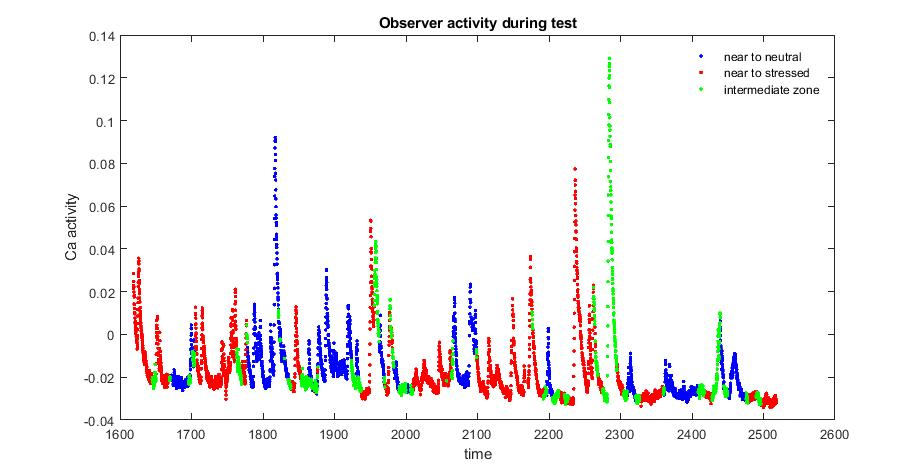
\includegraphics[scale=.60]{zone_plot.png} 
			\end{center} 
			\caption{zone plot function's output: different colors for different spatial positions}
		\end{figure}
		
		\item Next, I treated the issue of finding a way to establish weather a neuron is active or not, giving as result a binary matrix, 1 if activated or 0 if not at a specific time. A first naive way is using a treshold and considering active everything above it. this is what \textit{$activity\_detector$} does. With \textit{$detector\_plot$}, choosing the neuron you want to see as input, we can have a graphical explanation of this method (see Figure)
		
		\begin{figure}[H]
			\begin{center}
				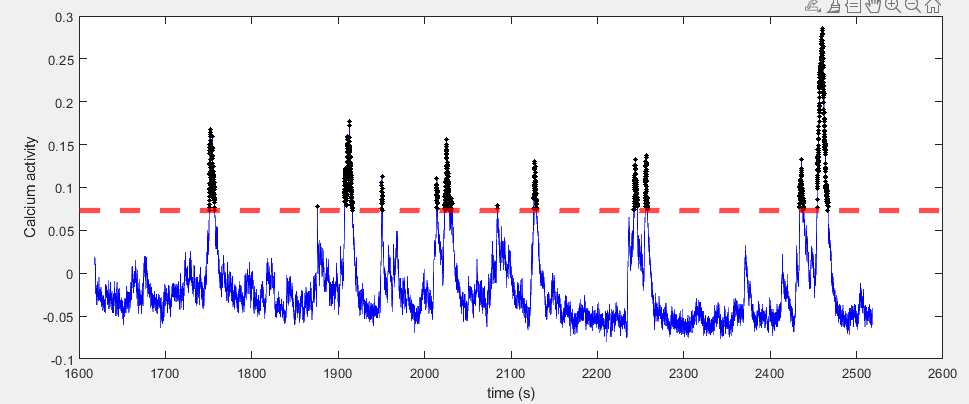
\includegraphics[scale=.60]{detector_plot.png} 
			\end{center} 
			\caption{Detector plot function's output: balck dots are neurons considered active. The treshold (in red) is given by $t = \mu + 2 \sigma$}
		\end{figure}
		
		\item With \textit{$mad\_tresh$} I started to work (not finished yet)  on a better tresholding system: I took inspiration from the median absolute deviation (mad) algorithm described at page 67-68 of the Inscopix manual. As we can observe in the figure, this new treshold is varying with the calcium activity, instead of being a straight line
		
		\begin{figure}[H]
			\begin{center}
				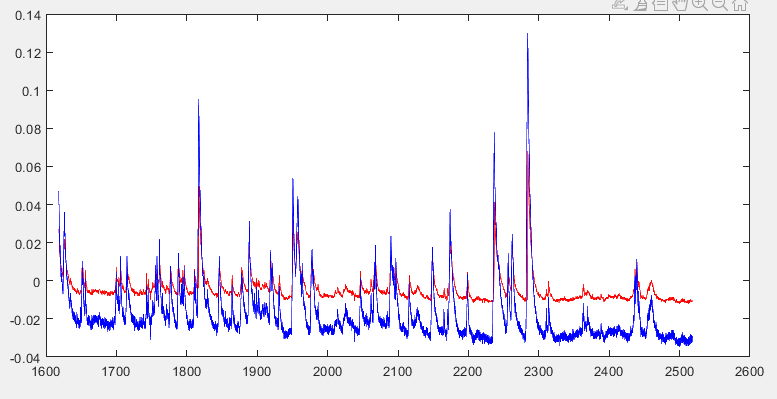
\includegraphics[scale=.60]{mad_plot.png} 
			\end{center} 
			\caption{plot mad function's output: the treshold (in red) is given by the curve obtained from mad algorithm}
		\end{figure}
		
		
		\item With the script \textit{$histograms$} we can observe the histograms of neurons activities in the 3 mice, to observe the activity mean and its distribution around it. it seems that Gamma probability densities (with parameters estimated by Matlab) can well approximate them.
		
		\item With the script \textit{$mean\_and\_var$} we can see the behaviour of the mean and variance from neuron to neuron
		
		\item With the function \textit{$plot\_correlation$} we have a heatmap plot of the Pearson's correlation between the columns of the data matrix passed as input (for example the neurons activities to inspect the correlation between neurons in one mouse) 
		
		
		\subsection{Discussion}
		
		During the report of the new scripts in Matlab, some comments have been made:
		
		\begin{itemize}
			
			\item We can improve the $3D$ plot of calcium activity vs space. Riccardo suggests to build a mesh covering the spatial boundary and to associate on it the calcium value. Greta suggests the use of a colormap to better capture the variations of calcium. An idea could be to add the time variable and seeing this heatmap in different snapshot over some time instants
			
			\item Greta wonders wether the change of directions of mice in the arena could tell us some interesting informations
			
			\item The correlation can be applied between two mice, considering their overall activity, to establish how much their activity are linked
			
			\item It will for sure be useful to add the sniff data, and relate many of the works illustrated so far with the direct interaction between two mice.
			
			
		\end{itemize} 
		
		
		\subsection{Next in line}
		
		Next work will be focused on:
		
		\begin{itemize}
			
			\item Finishing the mad detector algorithm and being able to return a binary matrix
			
			\item Improve many of the plots shown
			
			\item Work on the 3D plot as discussed
			
			\item Including the sniffing informations in the analysis
			
			\item As requested by Francesco Papaleo, focus the research on the interbrain, i.e. how activity and behaviour in one mouse are related to the ones in another, and investigate activity synchronizations.
			
			
		\end{itemize}
		
	\end{itemize}
	
	\newpage
	
	\section{Incontro 3 (27/10/2021)}
	
	\subsection{What has been done}
	
	First of all, I uploaded in the meeting folder in Dropbox, a beamer presentation resuming what has been done up to this point.
	Mainly, new things consisted in:
	
	\begin{itemize}
		\item Final time adapting which makes the events coherent with the information on the A key TTL provided in the sniff file: with the \textit{sniff\_adapting} script, the times of the 3 mice and of the sniffing informations become coordinated
		
		\item I ultimated the MAD treshold algorithm, with the function \textit{mad\_detector} it's possible to get the binary matrix corresponding to the signals activations
		
		\item With the script \textit{sniff\_plot} it is possible to observe the sniffing interactions during the test, marked with dots
		
		\item I started a new topic: correlation analysis. Following the Kingsbury article, Pearson and cross correlation have been used as measure of synchronization between signals. The first, however, express the \textit{linear} dependence of two quantities and it could be not particularly fit to our case (in the Kingsbury article, indeed, they show an increase of Pearson correlation, yet an increase leading to less than 0.3 correlation, not very meaningful). The cross correlation, on the contrary, seems the best tool to determine correlation between two signals.
		
		\item The two correlation are defined as it follows(in continue and discrete form for the cross one):
			$$ Corr_P(X,Y) = \frac{Cov(X,Y)}{\sigma_X \sigma_Y} $$
			
			$$  Corr_C(X,Y)  = X \star Y (t) = X(-t)*Y(t) = \int_{-\infty}^{\infty}X(t-\tau)Y(t) dt $$
			
			$$  Corr_C(X,Y)  = X \star Y (m) = \sum_{n=0}^{N-m-1} X_{n+m}Y_n  $$
			
			 In the figure an example of cross correlation behaviour: it is computed as function of the \textit{lags}. The peak of cross correlation corresponds to the delay between the signals, hence a peak near to 0 means that the 2 signals are alligned. Hence, a high (normalized) cross correlation is  suggested, beside from an appropriate level between [0,1], from the presence of  a possible unique peak corresponding to the allignment of signals.
			 
			 	\begin{figure}[H]
			 	\begin{center}
			 		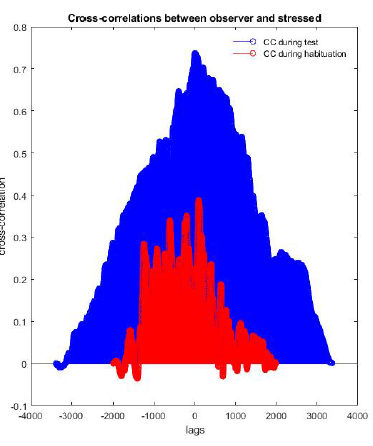
\includegraphics[scale=.90]{cross_corr.png} 
			 	\end{center} 
			 	\caption{Cross correlation between observer and stressed mice during test (blu) and habituation (red). We can observe a nice behaviour of the correlation for the test, compared to a no correlation behaviour in the habituation. This is reasonable: the correlation during the test is computed over times where observer and stressed were actually close, while during the habituation demonstrator mice are not present, and no correlation should be manifested}
			 \end{figure}
		 
		 \item For both the couples observer-stressed and observer-neutral, the test phase shows an increased cross correlation w.r.t the habituation phase. Moreover, if we restrict even more the times of interest to the one when actual sniffing happened, the cross correlation between observer and stressed (but not observer and neutral) is the highest recorded (see Figure)
		 
		 \begin{figure}[H]
		 	\begin{center}
		 		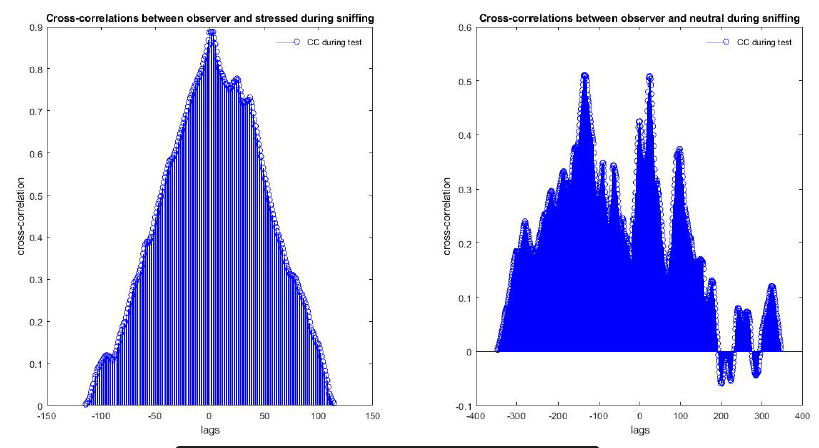
\includegraphics[scale=.70]{cross_corr_sniff.png} 
		 	\end{center} 
		 	\caption{Cross correlation between observer and stressed (left) and observer and neutral (right) during sniffing activities}
		 \end{figure}
	 
	 \item The next analysis focused instead on looking for correlations between single neurons activity: for every couple of neurons from one mouse and another, the cross correlation between the 2 signals has been computed and showed in a heatmap matrix. We can identify more clearly the couples showing synchronization coloring only the ones with a correlation above a certain treshold (I selected 0.6). Both for the matrices of the couples observer-stressed and observer-neutral, during the test phase the number of pairs showing correlation is significantly higher than during the habituation (see Figure)
	 
	 \begin{figure}[H]
		\begin{center}
			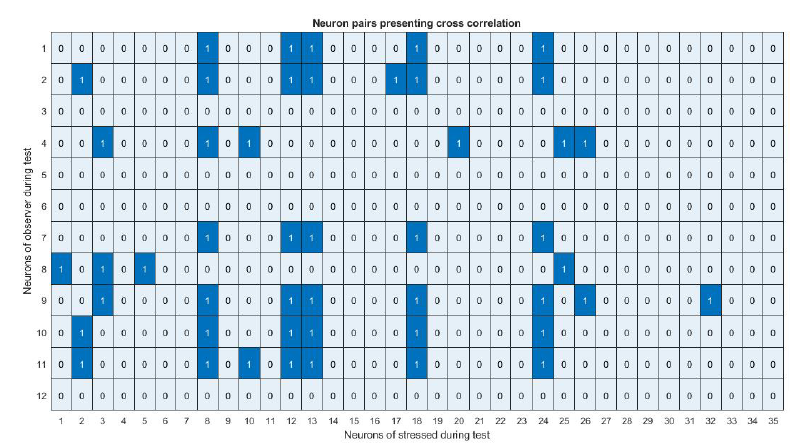
\includegraphics[scale=.60]{matrix_corr1.png} 
		\end{center} 

	\begin{center}
		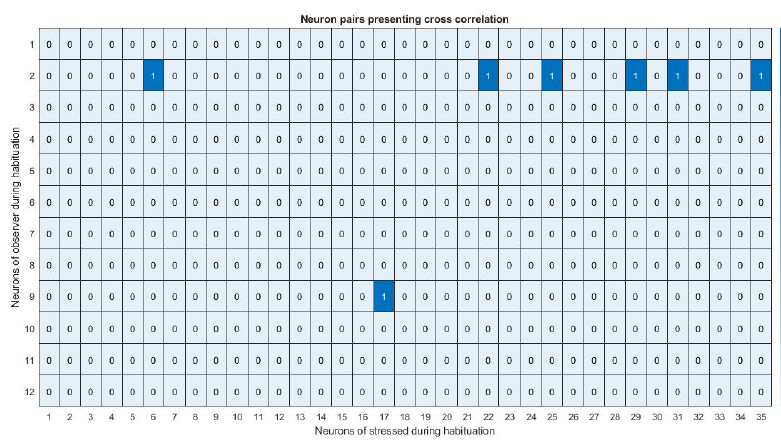
\includegraphics[scale=.60]{matrix_corr2.png} 
	\end{center} 
	\caption{	Synchronized pairs during test (top) and habituation (bottom). Similar results obtained both for observer vs stressed and observer vs neutral}

\end{figure}
	 			
	 	
	 
	 \item The latter analysis allows also to establish, for every mouse, which neurons are the ones "dedicated" to the correlation. Interestingly, for the observer the same neurons showed correlation with both the stressed and the neutral, even if coming from separate analysis
	 
	\end{itemize}
	
	
		\subsection{Fiberphotometry}
		
		
	Beside the Inscopix procedure to detect single neurons calcium activity, there is a second technique which will be object of work: \textbf{fiberphotometry}.
	A short guide on what fiberphotometry is can be found at \\ https://www.mightexbio.com/fiber-photometry/	\\
	In short, it is a technique consisting in a light stimultation and light emission in the brain resulting in a collective information on the mouse neural activity. There are not anymore single neurons informations, but only an overall intel, but this technique is faster, less invasive and cheaper. In the following I will start to work on Matlab also for the data coming from it (TBC).
	
	
		\begin{figure}[H]
		\begin{center}
			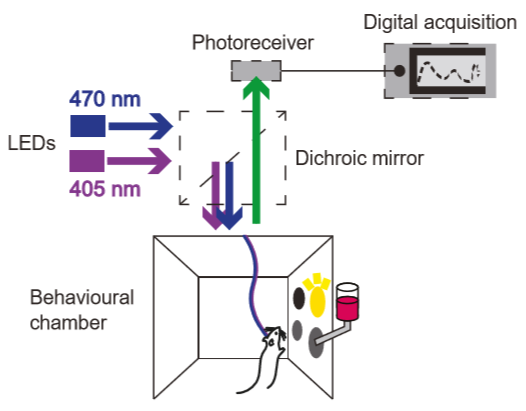
\includegraphics[scale=.60]{fiberphotometry.png} 
		\end{center} 
		\caption{Fiberphotometry experiment's setup: see the link for more}
	\end{figure}
	
	\subsection{Discussion}
	
	The discussion has been focused mostly on the first steps to follow in the differential modeling part, to be added to the data analysis part in the final work. Some discussions on:
	
	\begin{itemize}
		
		\item The difficulty in costructing a single cell model for the calcium activity, both for a non sufficient spatial resolution of the Inscopix microscope, both for the difficulty on establish the boundary conditions for a model of that type in relationship with the mouse behaviour during the experiment
		
		\item As consequence, it may be wiser to focus instead on the  neuron's network, focusing on the calcium activity patterns and electrophysiological links between neurons through axons
		
		\item As Riccardo suggests, the network could be threated as a collections of cables pairing single neurons. For every neuron of the network, the Ca activity is given by the experiment, and if we manage to find a link between calcium activity and membrane potential, the first one can be threated as boundary condition for a cable equation problem. A model of this type would then predict the potential drift along the network, and its link with the calcium activity for every single neuron
		
		\item Fabrizio suggests a couple of mathematical tools which may be helpful in an analysis of this type: \\
		Quantum graphs (https://en.wikipedia.org/wiki/Quantum\_graph) \\
		Differential models on networks (chapter 10 of the online interactive book by Barabasi - Albert may be useful: http://www.networksciencebook.com/chapter/10\#network-epidemic)
		
		\item Riccardo proposes a 2D model for the occupation probability of the observer in the arena (see the \textit{Sacco\_modello2D} file in the meeting folder)
		
		
		
	\end{itemize}
		
		
			\subsection{Next in line}
		
		Some IIT researchers asked me for help with Matlab on some codes related to fiberphotomety for thier experiments. Helping them should also help me to get familiar with this new technique. \\
		New data will come and the same correlation analysis will be tested on them, with the strong hope that similar results will be concluded (and start to be closer to an actual scientific result).\\
		Finally, more time will be dedicated on the differential model. For all of these reasons, for the time being I won't have time to go further on the data analysis, altough many things could still be done, they have to be postponed.
		
		\newpage
		
		\section{Incontro 4 (11/11/2021)}
		
		
		\subsection{Altruism experiment}
		
		I have been working also on a different experiment of fiberphotometry: \\
		
		\begin{figure}[H]
			\begin{center}
				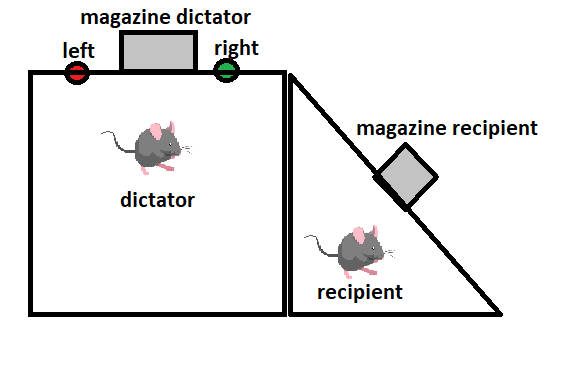
\includegraphics[scale=.90]{altruism.png} 
			\end{center} 
			\caption{Summarizing picture of the altruism experiment}
		\end{figure}
		
		We have a dictator and a recipient mouse. The dictator can stick his nose into two pokes to obtain pellets (i.e very yummy food :P). One poke is classified as selfish, since it will provide the pellet only through the magazine located in the dictator zone, while the other poke is altruist, since both in the dictator's magazine and in the recipient's will appear the pellet. This experiment is repetaed both with same and different pair of mice and during different days, randomizing every day the position of the selfish and altruistic poke. \\
		A dictator is classified as altruist if it shows a preference for the altruistic poke, which maintains for at least 3 days in a row, otherwise is classified as selfish.\\
		The goal of the experiment is to record the dictator's activity in the amigdala through fiberphotometry, observing the distinctions between selfish and altruistic mice during selfish and altruistic pokes. A distinction during first, intermediate and last days of the experiment is provided as well.
		\\
		Starting from pre-existent Matlab scripts, my job was to provide plots of the different situations from averages of different groups.
		
		\begin{figure}[H]
			\begin{center}
				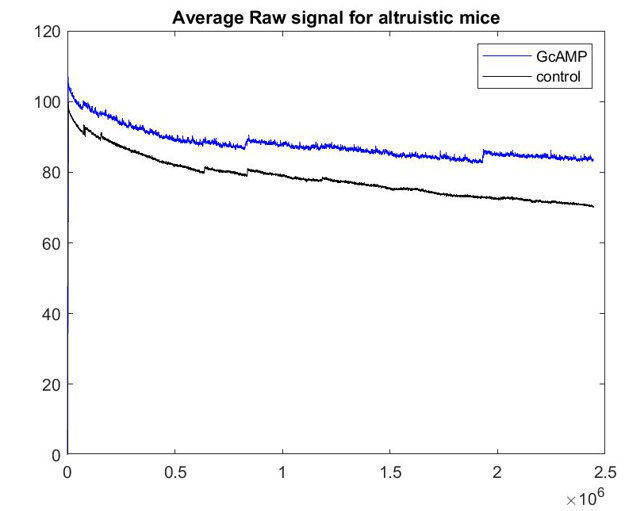
\includegraphics[scale=.60]{raw_signal.png} 
			\end{center} 
			\caption{Example of Average raw signal for a class of mice}
		\end{figure}
	
	 An important analysis has been the one of the \textbf{peri stimulus time istogram (PSTH)}, where we observe the change of the signal normalized on a baseline activity (first part of the test).
	 
	 \begin{figure}[H]
	 	
	 	\begin{center}
	 		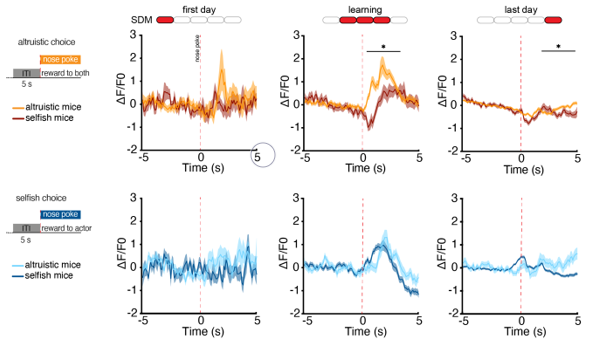
\includegraphics[scale=.99]{psth.png} 
	 	\end{center} 
	 	\caption{PSTH plot: the lines are the mean in the selected category, the colored fillings are the standard deviations (in red for selfish poke, in green for altruistic)}
	 	
	 \end{figure}
 
 \newpage
		
		
	\subsection{Development of a mathematical model}
				
				
In parallel to the data analysis, it would be nice to develop our own differential model. The main idea would be to work on the neuron network in the ROI. \\
We have information about posotion $(x,y)$ of every neuron, as well as their calcium activity along time. This suggests, as first thing to do, to investigate patterns in the calcium firing of neurons, possibily relating it to their distances. \\
To then build a model, we could consider on this neuronal network the propagation of the membrane potential described through PDEs in every link between neurons, and then simulate the overall firing dynamics in the ROI. There are, however, two main problems:

\begin{enumerate}
	
	\item Our data concern calcium activity, which we know for every neuron, while it's very unlikely to obtain the correct action potential from the microscopic cell's structure as done in electrophysiology differential models. Therefore, what we need here is a connection between the Calcium activity and the action potential in a cell. Approximations may be useful: we can see the calcium wave as a step function (with amplitude the max amplitude of the signal), and give it as buondary condition to the cable equation.
	
	\item The biggest problem is that in this network, we actually have no information about the adjacencies: we only have the nodes (neurons), but a priori we do not know if or when two neurons are connected or directly connected by a physical axon.\\
	A solution for this could be to not care about this in the model, but instead try to do a "calibration", which, based on the data we have of patterns in firing, will tell us how likely is that a possible connection between two neurons is actually there, or at least does the work for our model compared to reality. This could lead to a cable equation with varying conducibility.
	
	
	
\end{enumerate}		

If such calibration works, we would have created ourselves the preferentials arcs between neurons, and we could test the model on different firing patterns (which could be evaluated experimentally in the lab).\\
For example, a model describing the propagation of the action potential from neuron A ( with concentration $[Ca_A^{2+}](t)$) to neuron B ( with $[Ca_B^{2+}](t)$ ) may be given by : 

\begin{figure}[H]
	
	\begin{center}
		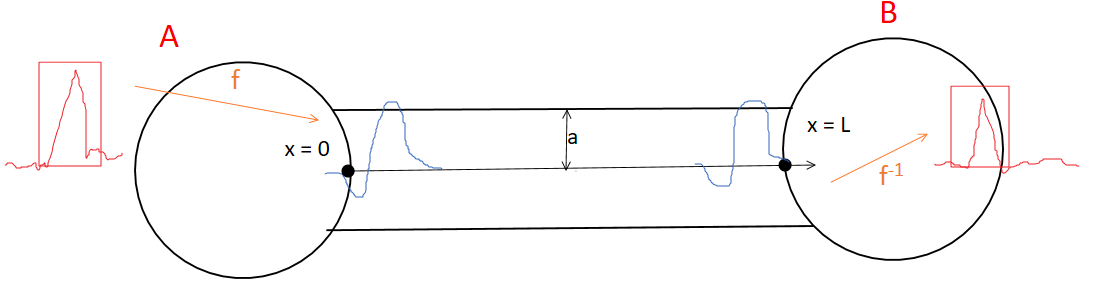
\includegraphics[scale=.55]{cable.png} 
	\end{center} 
		
\end{figure}
				
			\begin{Large}
				$$\begin{cases} 
				c_m \frac{\partial \psi}{\partial t} + \frac{1}{2 \pi a} \frac{\partial}{\partial x}\left(-\sigma \frac{\partial \psi}{\partial x} \right) = 0 & \text{in} \hspace{0.07 cm} (0,L) \times (0,T) \\
				\psi(0,t) = f([Ca_A^{2+}](t)) & \text{in} \hspace{0.07 cm} \left\{ x = 0\right\} \times (0,T) \\
				\psi(L,t) = f([Ca_B^{2+}](t)) & \text{in} \hspace{0.07 cm} \left\{ x = L\right\} \times (0,T) \\
				\psi(x,0)=0  & \text{in} \hspace{0.07 cm}  (0,L) \times \left\{ t = 0\right\}
				\end{cases}$$
			\end{Large}	
				
				
	Where the quantities $c_m$ (specific capacitance) and $a$ (axon radius) can be given by experimental values, while the conductance $\sigma$ can be link-specific.\\
	Finally, notice that:
	
	\begin{itemize}
		
		\item Instead of a B.C. on $x=L$ for the potential, we might want to compute it a posteriori and confront it, after having applied $f$, with the calcium activity in B: therefore, we can think on a different B.C., for example on the current at that point, as suggested by Riccardo
		
		\item The conducibility $\sigma$ is probably, from a biological point of view, constant for every link, we can consider it not constant to supply the lack of knowledge in the network. We can also think to keep it constant and give a preference for an arc instead of another based on another quantity (for example a probability computed from the available data)
		
		\item Since the r.h.s of the main equation is zero, in this assumption the cable is perfectly isolant, hypothesis which can be clearly modified if evidence shows otherwise. Same for the initial condition.
	\end{itemize}
	
	\subsection{Next in line}
	
	Next work will be focused on:
	
	\begin{itemize}
		
		\item Statistical analysis of the results obtained in the altruism experiment
		
		\item pattern identification in the calcium firing of the neurons in the ROI
		
		\item Research from the literature of the function (or else) linking calcium with potential
		
		\item Start of a simplified model of 2 neurons (such as in the picture), where the computed $\psi$ at $x = 0 $ and $ x = L$ and the calcium firing in A and B are coherent
	\end{itemize}
	
	\newpage
	
	\section{Incontro 5 (25/11/2021)}
	
	
	\subsection{Analysis of new datasets}
	
	Datasets III and IV have been studied (for a detailed presentation of the results, see the document \textit{Beamer\_24\_November} in Meetings folder). \\
	These two new experiments had the same triplets of mice in experiments I and II, but this time the observers have been previously stressed.
	As showed in the following figures, both for dataset III and IV, in counterposition to the first two datasets, no correlation seems to arise between both pairs of mice, considering their vicinance during the all test: no significant difference is manifested between habituation and test, and the correlation peak is significantly smaller.
	
	
	
	\begin{figure}[H]
		\begin{center}
			\hspace*{-1cm}
			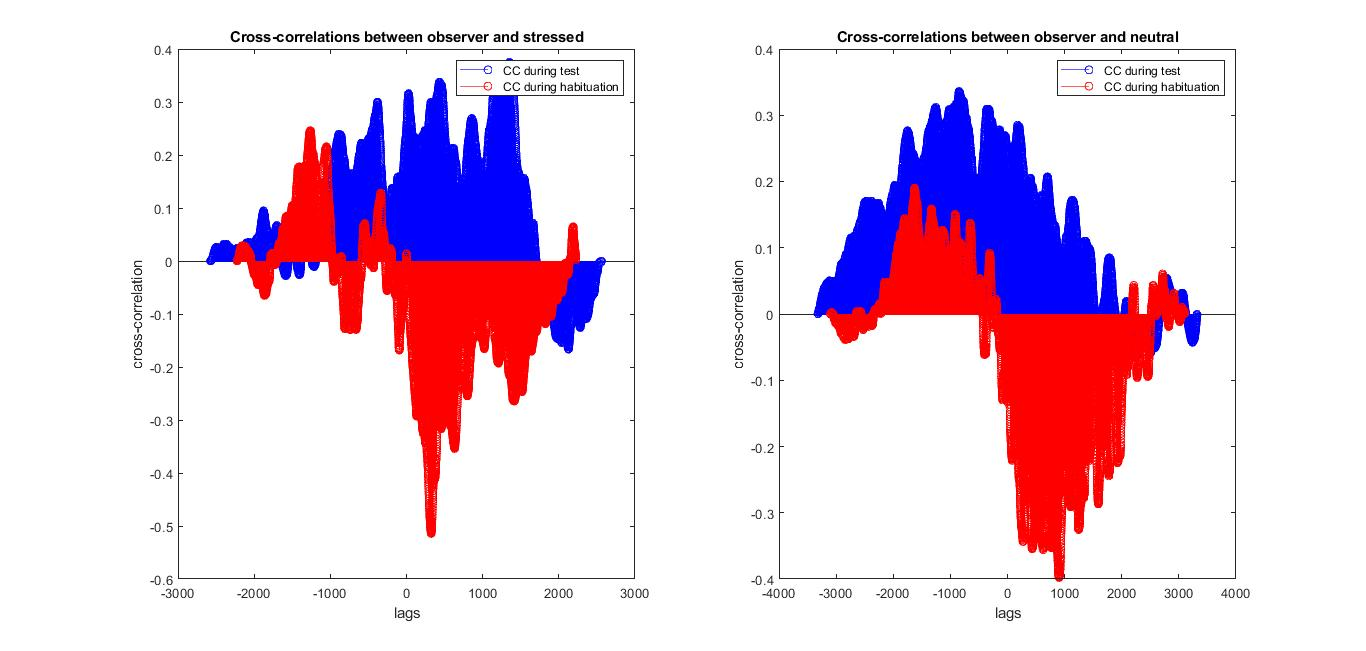
\includegraphics[scale=.36]{obs_stress_neut.jpg} 
		\end{center}  
	\caption{Cross correlations in III dataset}
	\end{figure}
	
	
	\begin{figure}[H]
		\begin{center}
			\hspace*{-1cm}
			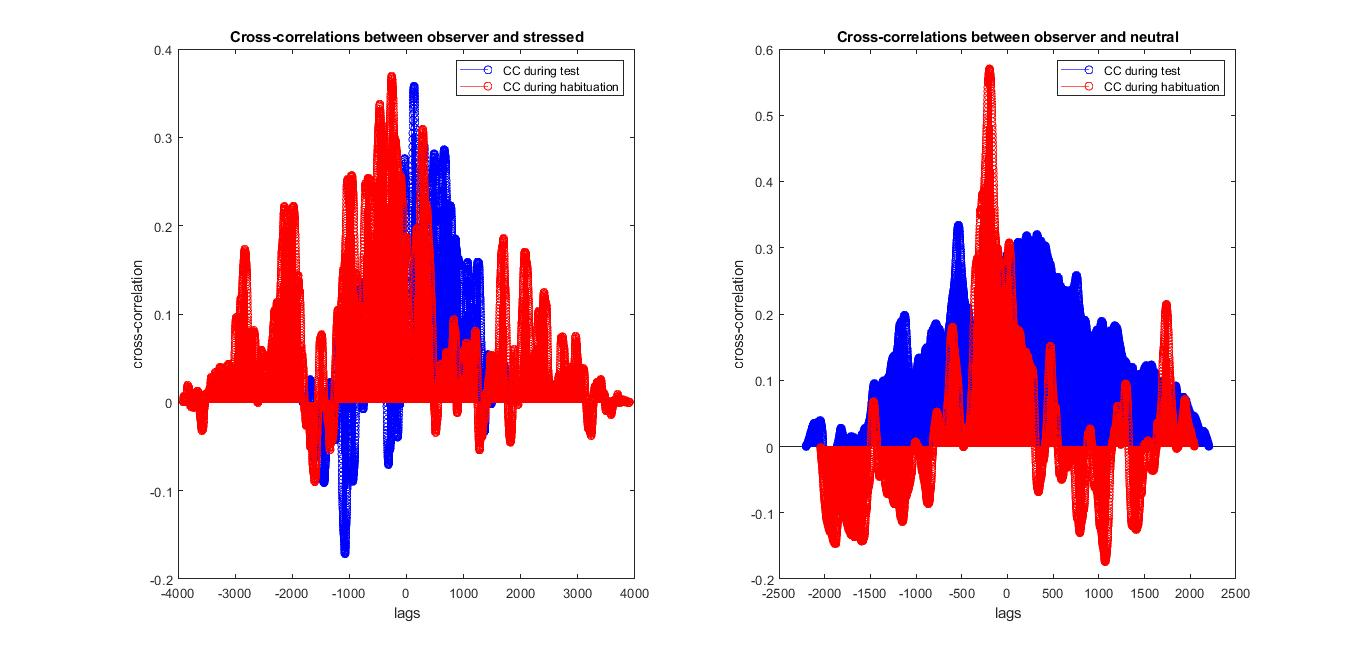
\includegraphics[scale=.32]{obs_stress_neut4.jpg} 
		\end{center}  
		\caption{Cross correlations in IV dataset}
	\end{figure}
	
	
	
	However, an analysis of the activity correlation during sniffing reveals a high correlation for the III dataset between observer and stressed (data not available for IV dataset).
	
	
	\begin{figure}[H]
		\begin{center}
			\hspace*{-1cm}
			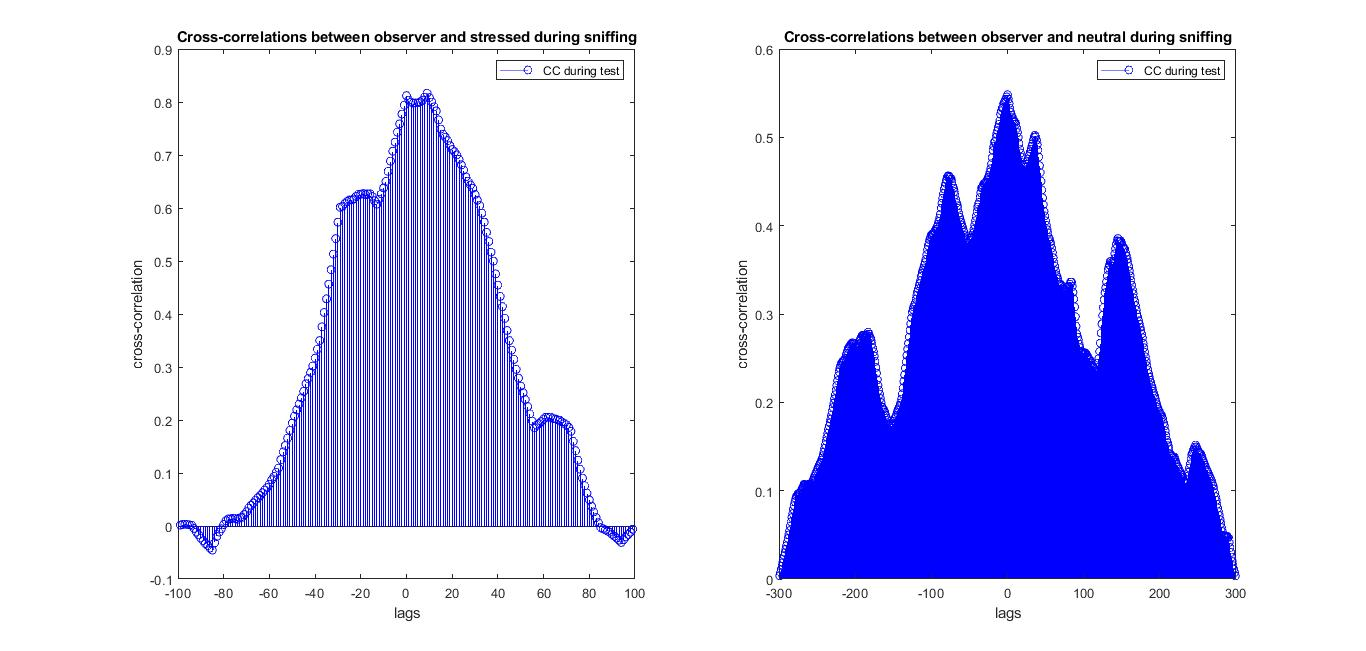
\includegraphics[scale=.32]{sniff3.jpg} 
		\end{center}  
		\caption{Cross correlations during sniffing in III dataset}
	\end{figure}
	
	
	
	
The result about single neuronal pairs correlation is even more surprising: in both datasets (especially IV), the percentage of synchronized pairs is way higher in the test rather than in habituation (however, see next comments on this coming soon). \\
	
As final analysis, I wanted to consider as well the change in correlation over time, namely if during the all period of vicinance, there are difference in the correlation of mice activities. For datasets I and II, between observer and stressed I found a slightly higher correlation in the first part of the test, but still a high correlation recorded during all test (and indeed the cc recorded during all test was high).


		\begin{figure}[H]
		\begin{center}
			\hspace*{-1cm}
			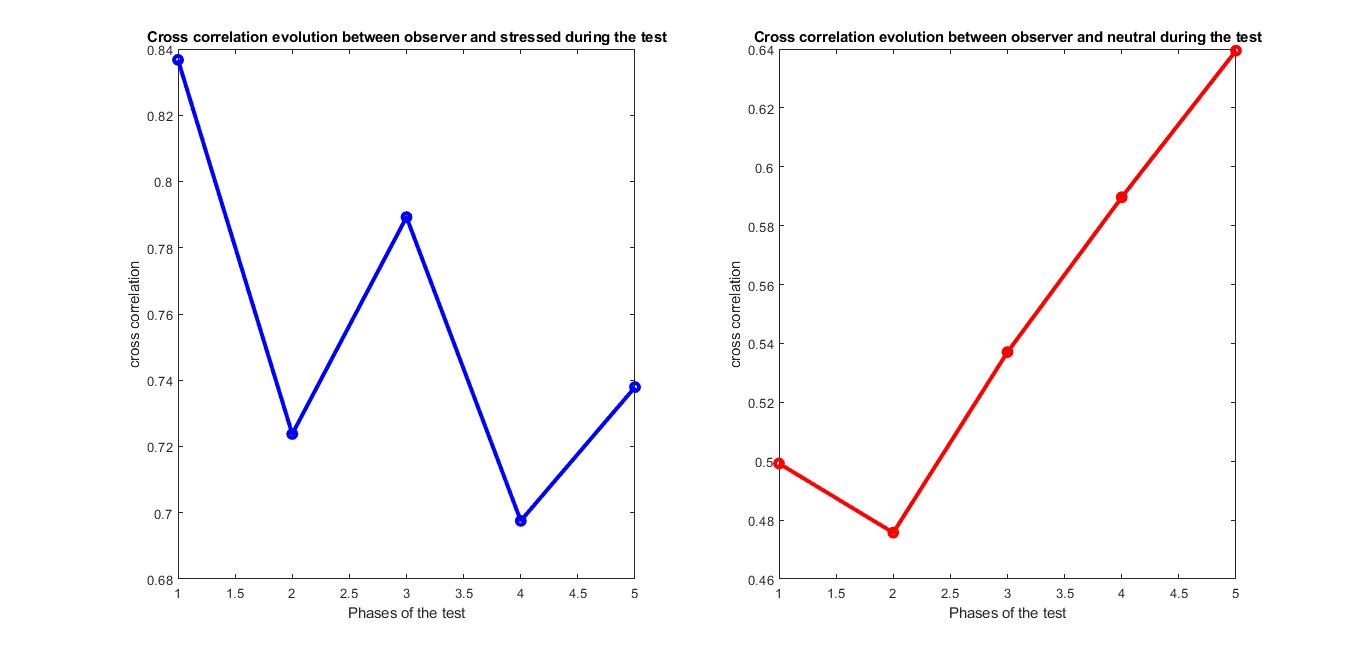
\includegraphics[scale=.36]{corr_time.jpg} 
		\end{center}  
		\caption{Cross correlations over time in I dataset}
		
	\end{figure}

		
		Also for dataset III  and IV (especially III, results in dataset IV are the less significant), in the first part the cc seems higher, but this time it goes faster to lower values, compromising the overall correlation measured during all test. This could suggest a "short memory" behaviour for observers when stressed. At this regard, it could be worth to notice that most of the sniffing between observer and stressed occured in the first half of the test, where cc is higher, and therefore could justify the higher peak on the correlation showed. Indeed, restricting the analysis of cc during sniffing at the first part of the test, we retrieve higher correlation both during vicinance of observer/stressed and observer/neutral, both during sniffing interactions.
		
		
			\begin{figure}[H]
			\begin{center}
				\hspace*{-1cm}
				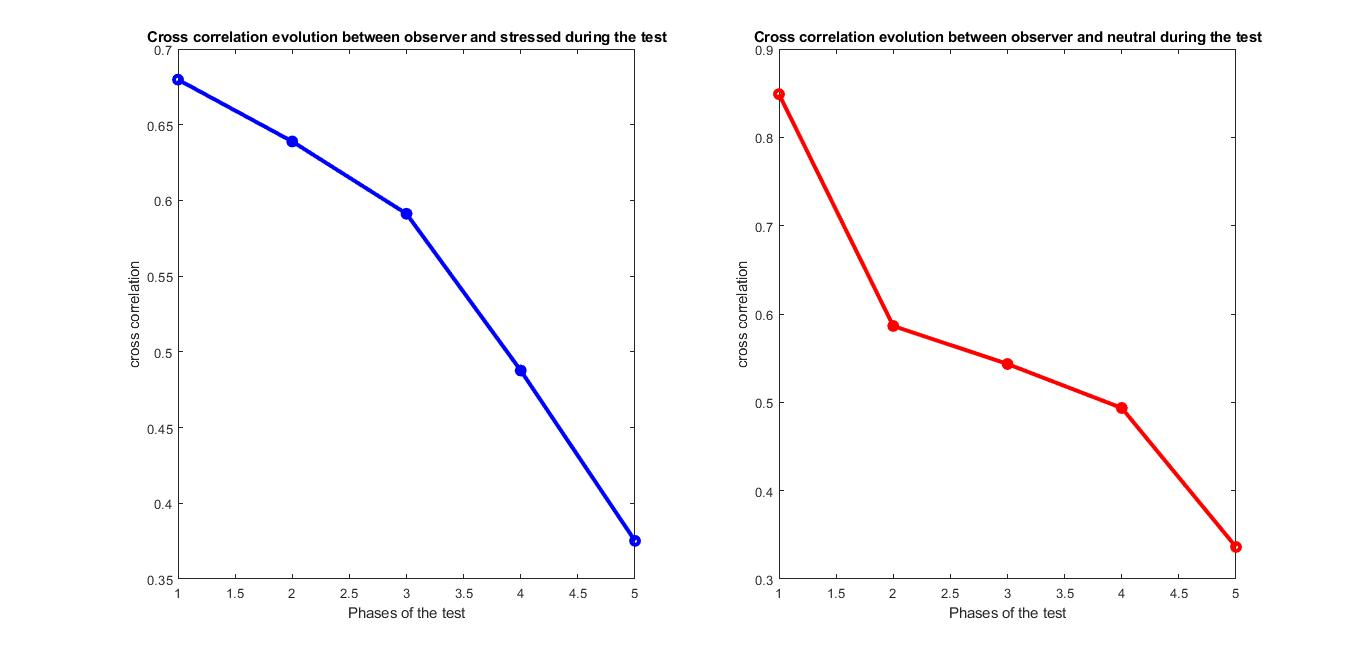
\includegraphics[scale=.36]{corr_time3.jpg} 
			\end{center}  
			\caption{Cross correlations over time in III dataset}
			
		\end{figure}
		
		
		
\subsection{Comments on obatined results}		
		
	\begin{itemize}
		
		\item Stressing the observer seems to annihilate the correlation observed in precedence during the all test. However, such correlation could still be present in the first parts of the test, to then vanish faster
		
		\item About the single neurons synchronization, maybe the cross correlation analysis is not the best choice: the behaviour of Ca oscillations observed in single neurons is more of the kind ON/OFF, with a baseline flat activity alterned to high and fast peaks. On the contrary, doing the average activity, the resulting signal is more homogeneous. therefore, cc analysis could be more optimal for the average signal rather than the singol neuronal one, where synchrinization could be studied instead based on the reciprical ON state of 2 neurons (TBC)
		
		\item I inspected also the $L^2$ and infinity errors between signals during the different phases (see slides)
		
		\item Average considerations on first two and last two datasets are shown in the following figures (see slides for more)
		
	\end{itemize}	
		
		
		
			\begin{figure}[H]
			\begin{center}
				\hspace*{-1cm}
				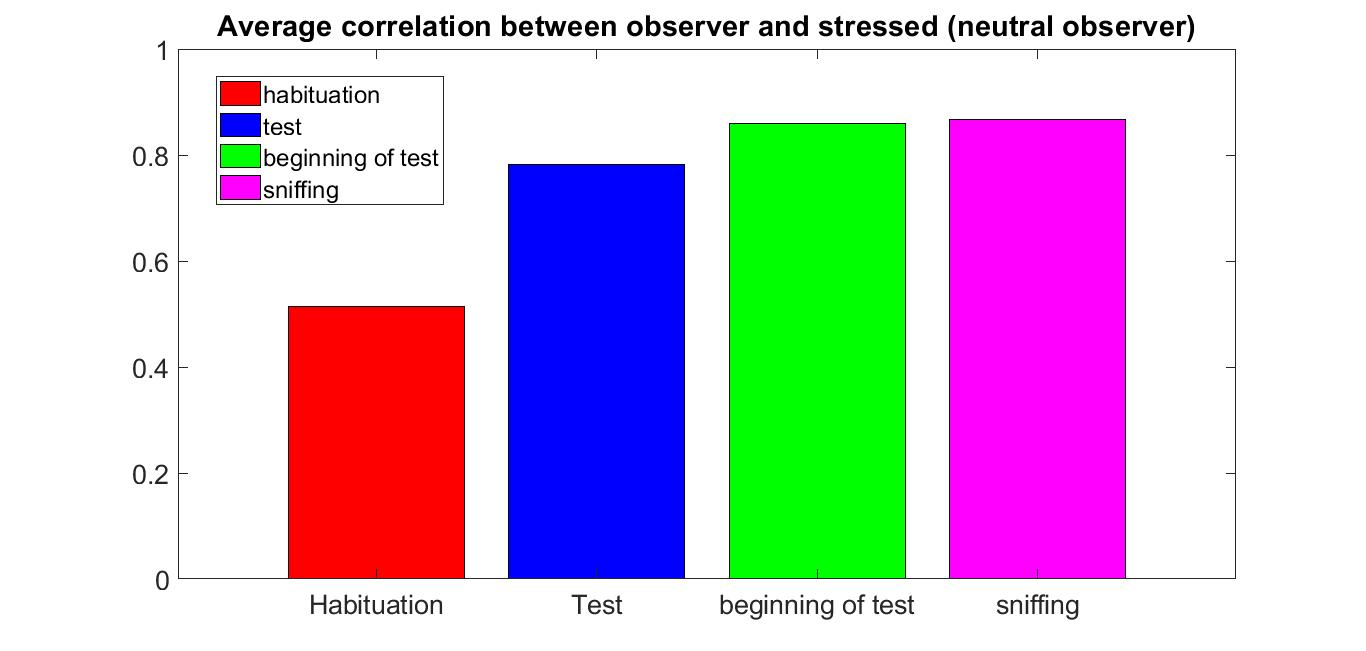
\includegraphics[scale=.36]{avg_corr_stress.jpg} 
			\end{center}  
			\caption{Average correlations between observer and stressed (datasets I and II)}
			
		\end{figure}
	
	
	\begin{figure}[H]
		\begin{center}
			\hspace*{-1cm}
			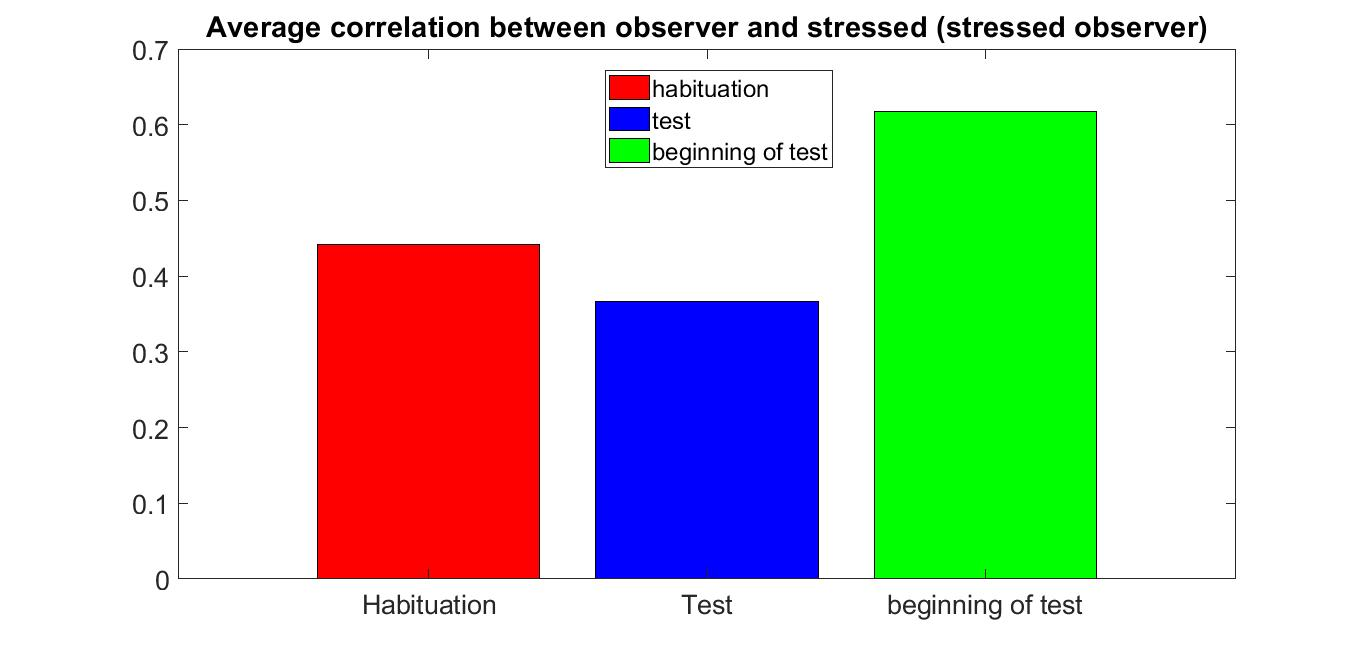
\includegraphics[scale=.36]{avg_corr_stress2.jpg} 
		\end{center}  
		\caption{Average correlations between observer and stressed (datasets III and IV)}
		
	\end{figure}
		
		
		\subsection{Discussion}	
		
	The discussion between Fabrizio and Riccardo has been mostly about the cable model to implement. A potentially helpful relationship between action potential and Ca activity can be found in the article by Koster and Sackmann (tjp file in Meetings folder). Here there is a formula connecting the amplitude $A_c$ of the calcium oscillation with the one $A_p$ of the action potential (if there is a train of $N$ AP waves with amplitude $A_p$):
	
	$$ A_c = A_p \sum_{i=0}^{N}e^{-\frac{t+i/f}{\tau}}  \hspace{1 cm} at  \hspace{0.5 cm} t=0 $$
		
		
	Several constants have to be estimated empirically / by experiments / from literature (see article for more).
	
	Once we have such relationship, we can obtained the boundary condition at $x=0$ of the 2 neurons model discussed in the previous meeting, retrieving $A_p(x=0)$ from the available  datum	$A_c$ of neuron A, then simulate the cable equation and observe if, from the obtained amplitude $A_p(x=L)$, the quantity $A_c (x=L)$ obtained through the formula is coherent with the observed value in neuron B.
		
	\subsection{Next in line}		
		
		\begin{itemize}
			
			\item I will continue a work started on pattern recognition between neurons in a ROI, as well as neuronal synchronization of ON/OFF type discussed, and study of relationship between neurons patterns and interneurons distance
			
			\item New data with observers neutral and stressed will arrive to complete the picture of the two cases
			
			\item It's probably time to start the implementation of the 2 neurons cable model discussed
			
			\item The Genetics of cognition team will start a collaboration with an IIT laboratory in Rome held by Giacomo Novembre (https://www.giacomonovembre.com/). Apparently they are studying interbrain in humans (with different techniques). A meeting to discuss collaborations will come soon
			
			
		\end{itemize}
		
		
		
		
		
		
		
	
	
\end{document}






\section{Introduction}

\begin{figure}[H]
\begin{center}
	\includegraphics[scale=.40]{ad_stab.png} 
\end{center} 
\caption{\textit{Numerical solution (blu) and real solution (black) in the  stabilized case for advection-diffusion problem}}

\end{figure}